\PassOptionsToPackage{hyphens}{url} % break long URLs
\documentclass{prog_report}

\usepackage{url}
\usepackage{hyperref}
\usepackage{todonotes}

\newcommand{\footurl}[1]{\footnote{\url{#1}}}

\renewcommand{\baselinestretch}{1.0}

\begin{document}

\title{WASP Cloud Assignment – Project 1}

\author{Joel Scheuner (scheuner@chalmers.se), Joris Van Rooij (jorisv@chalmers.se)}
%\email{scheuner@chalmers.se}

\date{\today}

\maketitle

%You will write a report where you will explain your choice of the methods, and the dataset. You will describe your setup, and your conclusion. As scientists, you should be able to describe why you have reached that conclusion, e.g., by showing performance speedup graphs or slowdowns. Please comment on the behaviour you see, if it is linear in the amount of resources, sublinear, or something else, or if the CPU was the bottleneck, or the Memory, etc? 
%
%Please follow the data science process, and comment on how you have followed it.

This report presents the methodology and summarizes the results of \emph{project 1} for the WASP cloud assignment.

% In your report, include a link to your code on github. 
Github repo: \url{https://github.com/joe4dev/wasp-cloud-spark/}

\section{Methodology}

\subsection{Pyspark Libary}
We choose to evalute the methods \emph{multiply(other)} of the BlockMatrix and \emph{computeSVD(k)} of the IndexedRowMatrix in the distributed module of the LINALG Spark library (version 2.4.3) for Python (i.e., Pyspark)\footurl{https://spark.apache.org/docs/2.4.3/api/python/pyspark.mllib.html\#module-pyspark.mllib.linalg.distributed}.
Initially, we thought the Scala version of the library would be a good fit because Spark itself is written in Scala but we discovered a severe lack of documentation (particularly for the relevant distributed module) for the Scala\footurl{https://spark.apache.org/docs/2.4.3/api/scala/\#org.apache.spark.mllib.linalg.distributed.package} and Java\footurl{https://spark.apache.org/docs/2.4.3/api/java/} API documentation.
The Python API had least some documentation including a couple of code examples and direct links to the source code.
Based on the API documentation, we selected the following shortlist of non-trivial operations (e.g., excluding numRows(), transpose()):

\begin{itemize}
    \item
    \href{https://spark.apache.org/docs/2.4.3/api/python/pyspark.mllib.html\#pyspark.mllib.linalg.distributed.BlockMatrix.add}{add(other)}:
    ``The matrices must have the same size and matching rowsPerBlock and
    colsPerBlock values.''
    \item
    \href{https://spark.apache.org/docs/2.4.3/api/python/pyspark.mllib.html\#pyspark.mllib.linalg.distributed.BlockMatrix.multiply}{multiply(other)}:
    ``The colsPerBlock of this matrix must equal the rowsPerBlock of
    other.'' Better no SparseMatrix blocks because they have to be
    converted to DenseMatrix blocks, which may lead to performance
    issues due to lacking support for multiplying two sparse matrices.
    \item
    \href{https://spark.apache.org/docs/2.4.3/api/python/pyspark.mllib.html\#pyspark.mllib.linalg.distributed.BlockMatrix.subtract}{subtract(other)}:
    ``The matrices must have the same size and matching rowsPerBlock and
    colsPerBlock values.''
    \item
    \href{https://spark.apache.org/docs/2.4.3/api/python/pyspark.mllib.html\#pyspark.mllib.linalg.distributed.IndexedRowMatrix.computeSVD}{computeSVD(k,
        computeU=False, rCond=1e-09)}: ``Computes the singular value
    decomposition of the IndexedRowMatrix.''
    \item
    \href{https://spark.apache.org/docs/2.4.3/api/python/pyspark.mllib.html\#pyspark.mllib.linalg.distributed.IndexedRowMatrix.multiply}{multiply(matrix)}:
    ``Multiply this matrix by a local dense matrix on the right.''
    \item
    \href{https://spark.apache.org/docs/2.4.3/api/python/pyspark.mllib.html\#pyspark.mllib.linalg.distributed.RowMatrix.columnSimilarities}{columnSimilarities(threshold=0.0)}:
    ``Compute similarities between columns of this matrix.''
    \item
    \href{https://spark.apache.org/docs/2.4.3/api/python/pyspark.mllib.html\#pyspark.mllib.linalg.distributed.RowMatrix.tallSkinnyQR}{tallSkinnyQR(computeQ=False)}:
    ``Compute the QR decomposition of this RowMatrix. The implementation
    is designed to optimize the QR decomposition (factorization) for the
    RowMatrix of a tall and skinny shape.''
\end{itemize}

We decided to implement and evaluate the following two methods:
\begin{itemize}
    \item \code{pyspark.mllib.linalg.distributed.BlockMatrix.multiply(other)}
    \item \code{pyspark.mllib.linalg.distributed.IndexedRowMatrix.computeSVD(k)}
\end{itemize}
We choose these methods because they are implemented for the distributed matrix types of \emph{BlockMatrix} and \emph{IndexedRowMatrix}, which is beneficial for distributed computing.
Further, multiply seems the de-facto standard for benchmarking matrix operations in practice (e.g., also used in the pull request contributing to the distributed Spark module\footurl{https://github.com/apache/spark/pull/2294}).
Finally, computeSVD has been described in literature as one "of the more interesting approaches"\cite{bosagh-zadeh:16}:

\subsection{Dataset Choice}

Following the task description, we selected an appropriate matrix dataset from the "SuiteSparse Matrix Collection"\footurl{https://sparse.tamu.edu/}.
We use the \code{.mtx} Matrix Market format as it can be easily parsed using the popular Python SciPy\footurl{https://www.scipy.org/} library.
For the actual evaluation, we chose a sparse matrix of size 3140 by 3140 with 543,160 nonzero values. 
Tests performed with Spark on a single laptop showed reasonable runtimes for the selected calculations with this matix.
The SciPy method \code{mmread} transforms the matrix in a format that allows extraction of it rows. 
An enumeration of these rows was used to create the Spark RDDs with indexed rows. 
The number of RDDs created seemed to be influenced by the \emph{numSlices} parameter, which in turn influences the processing speed and scalability of the computations.
Some experimentation showed that a value of 512 resulted in swift computation and good scalability.
The RDDs with indexed rows were used to create a distributed \emph{IndexedRowMatrix}, which in turn could be transformed in a \emph{BlockMatrix}. 

\subsection{Google Dataproc Cloud Platform}

Following the task description, we use the cloud-native Apache Spark infrastructure Google Dataproc\footurl{https://cloud.google.com/dataproc/}.
Dataproc offers several API interfaces\footurl{https://cloud.google.com/dataproc/docs/api-libraries-overview} based gRPC\footurl{https://grpc.io/} including client SDKs in many languages and a command line interface called gcloud.
We wanted to automate the creation of different-sized clusters to conduct the performance speedup analysis and therefore choose to explore the Python API\footurl{https://googleapis.github.io/google-cloud-python/latest/dataproc/index.html} instead of writing shell scripts for the gcloud CLI.
This also seemed a reasonable choice as our computation code is already written in Python.
There is some introductory documentation\footurl{https://cloud.google.com/dataproc/docs/tutorials/python-library-example} and a Github repository with Python examples\footurl{https://github.com/GoogleCloudPlatform/python-docs-samples/tree/master/dataproc} available.
However, we figured out that the Python API is just in alpha status and documentation in the API reference\footurl{https://googleapis.github.io/google-cloud-python/latest/dataproc/gapic/v1/api.html} is practically inexistent.
Even fundamental cluster configuration options were basically undocumented and had to be reverse-engineered from the gRPC Dataproc API\footurl{https://cloud.google.com/dataproc/docs/reference/rpc/google.cloud.dataproc.v1\#google.cloud.dataproc.v1.ClusterConfig} or the actual source code.
Even worse, essential configurations, such as installing pip dependencies using the out-of-the-box Python initialization actions\footurl{https://github.com/GoogleCloudPlatform/dataproc-initialization-actions/tree/master/python}, were impossible due to gRPC request validity restrictions (e.g., it was impossible to set uppercase environment variables using metadata because only lowercase metadata keys were allowed).
We had to find several workaround for such issues but finally managed to implement a Python orchestrator script that creates a cluster and necessary Google storage buckets, submits a pyspark job multiple times, automatically resizes the cluster (i.e., by adding extra nodes), and finally deletes the cluster.
The cluster resizing operation is particularly interesting (and particularly poorly documented) as it allows us to adjust the number of worker nodes without having to re-create the entire cluster.

For monitoring the cluster during job execution, we created a Stackdriver\footurl{https://cloud.google.com/stackdriver/} account.
Stackdriver integrates seemlessly into Google Dataproc and provides charts of CPU utilization, memory allocation, network I/O, disk I/O, etc.

\section{Results and Discussion}

%As scientists, you should be able to describe why you have reached that conclusion, e.g., by showing performance speedup graphs or slowdowns. Please comment on the behaviour you see, if it is linear in the amount of resources, sublinear, or something else

Figure~\ref{fig:multiply} shows ...

%\begin{figure}
%    \centering
%    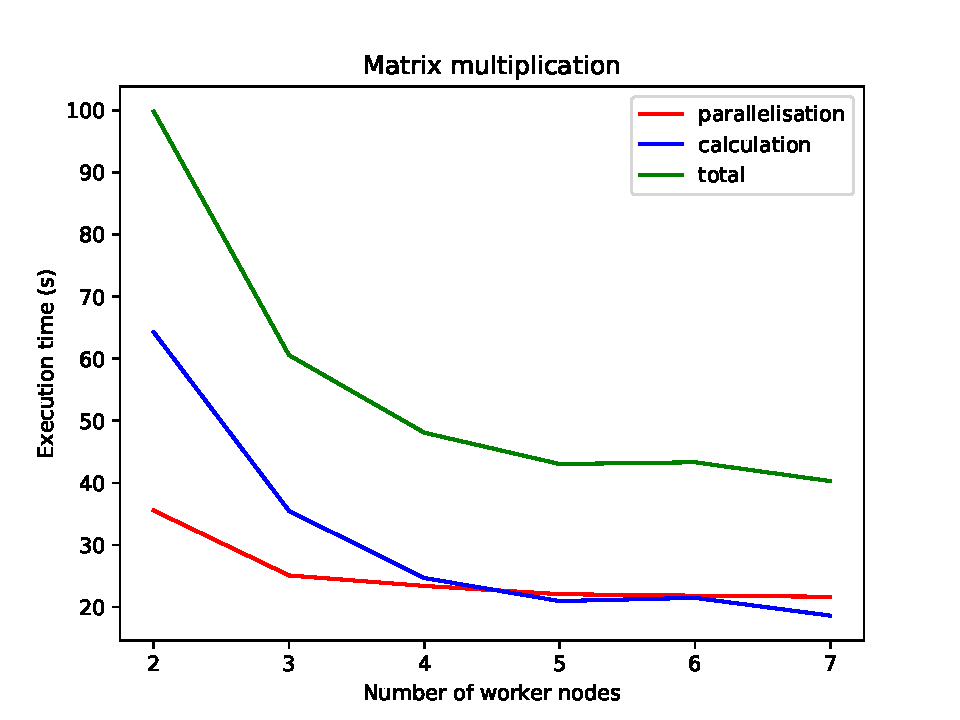
\includegraphics[width=\textwidth]{img/multiply-speedup}
%    \caption{Multipy Method – Speedup}
%    \label{fig:multiply}
%\end{figure}

The summary of monitoring charts in Figure~\ref{fig:multiply-charts} reveals that CPU utilization seems to be the the limiting factor of the matrix computation jobs as indicated by peaks above 0.8 reaching almost full utilization 1.0 at the end of the experiment.
Figure~\ref{fig:multiply-cpu} and Figure~\ref{fig:multiply-mem} detail the actual CPU and memory utilization of the cluster during the approximately one hour experiment.

\begin{figure}[h]
    \centering
    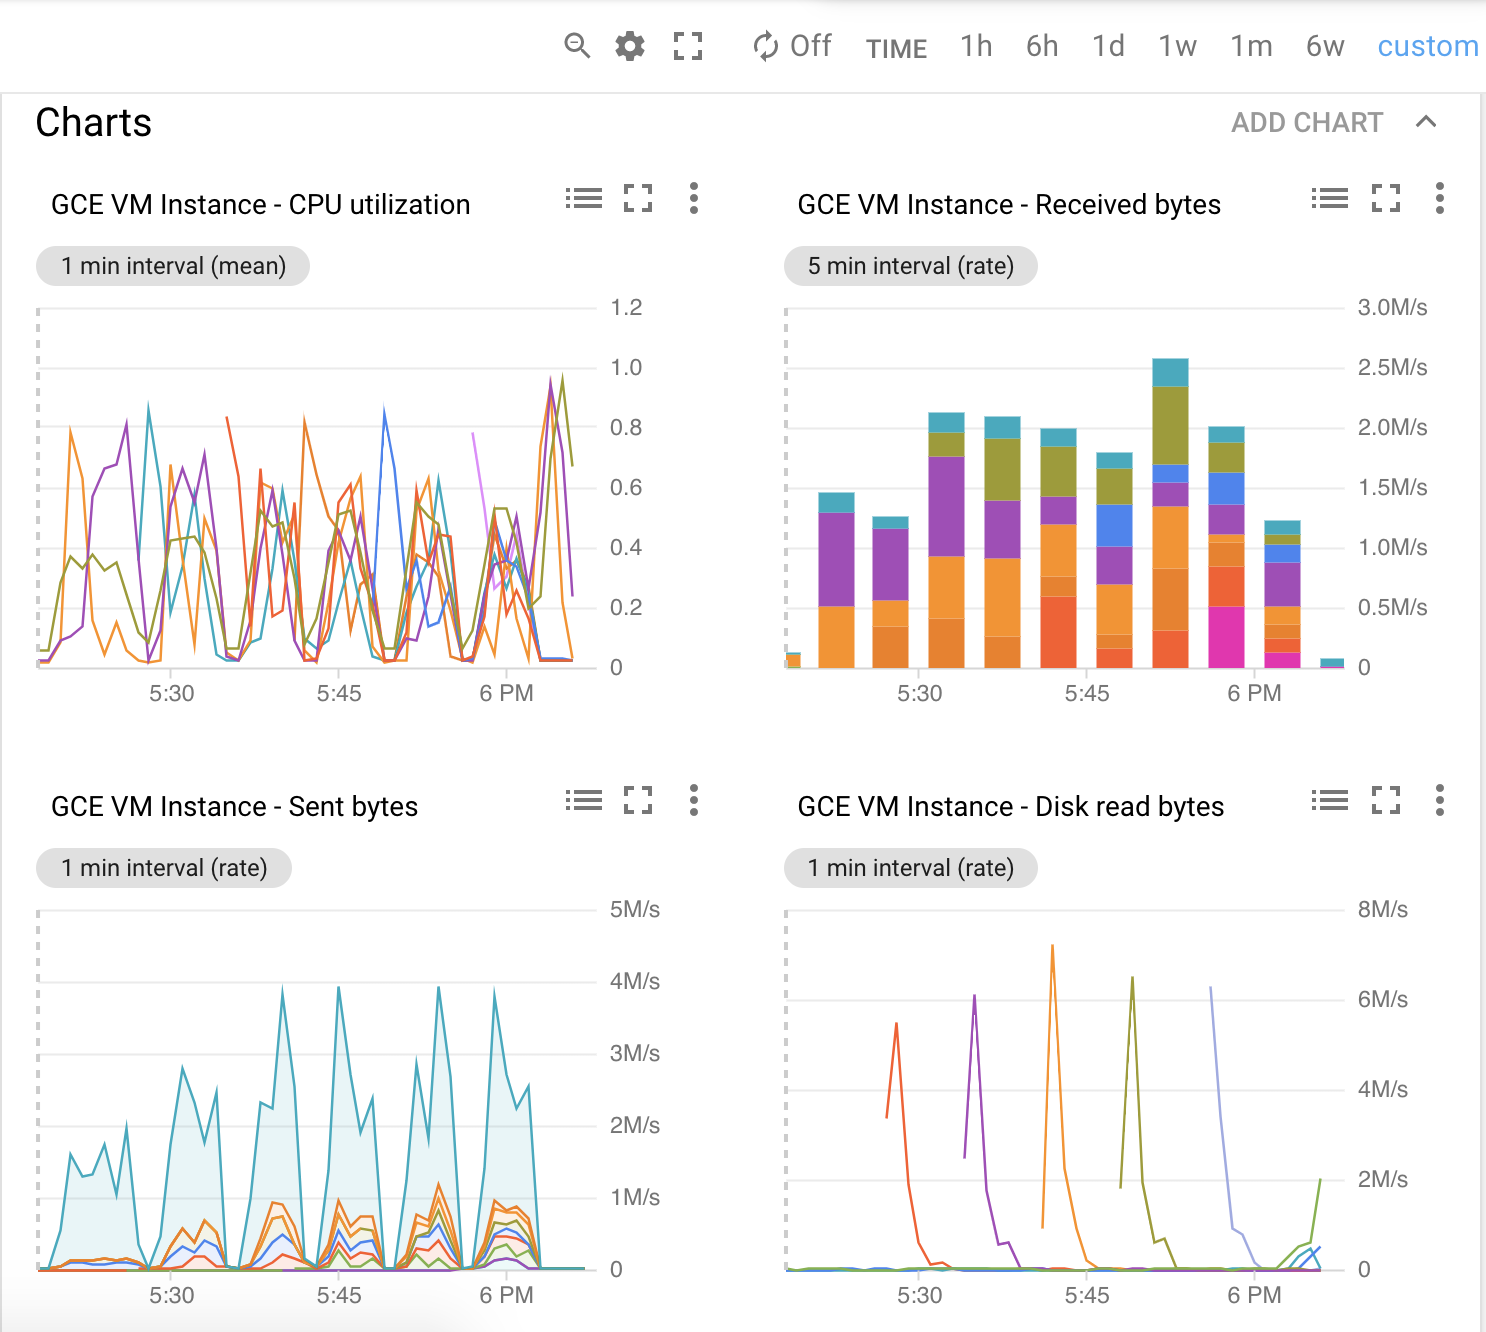
\includegraphics[width=0.8\textwidth]{img/multiply-resources}
    \caption{Multipy Method – Resource Utilzation}
    \label{fig:multiply-resources}
\end{figure}

\begin{figure}[h]
    \centering
    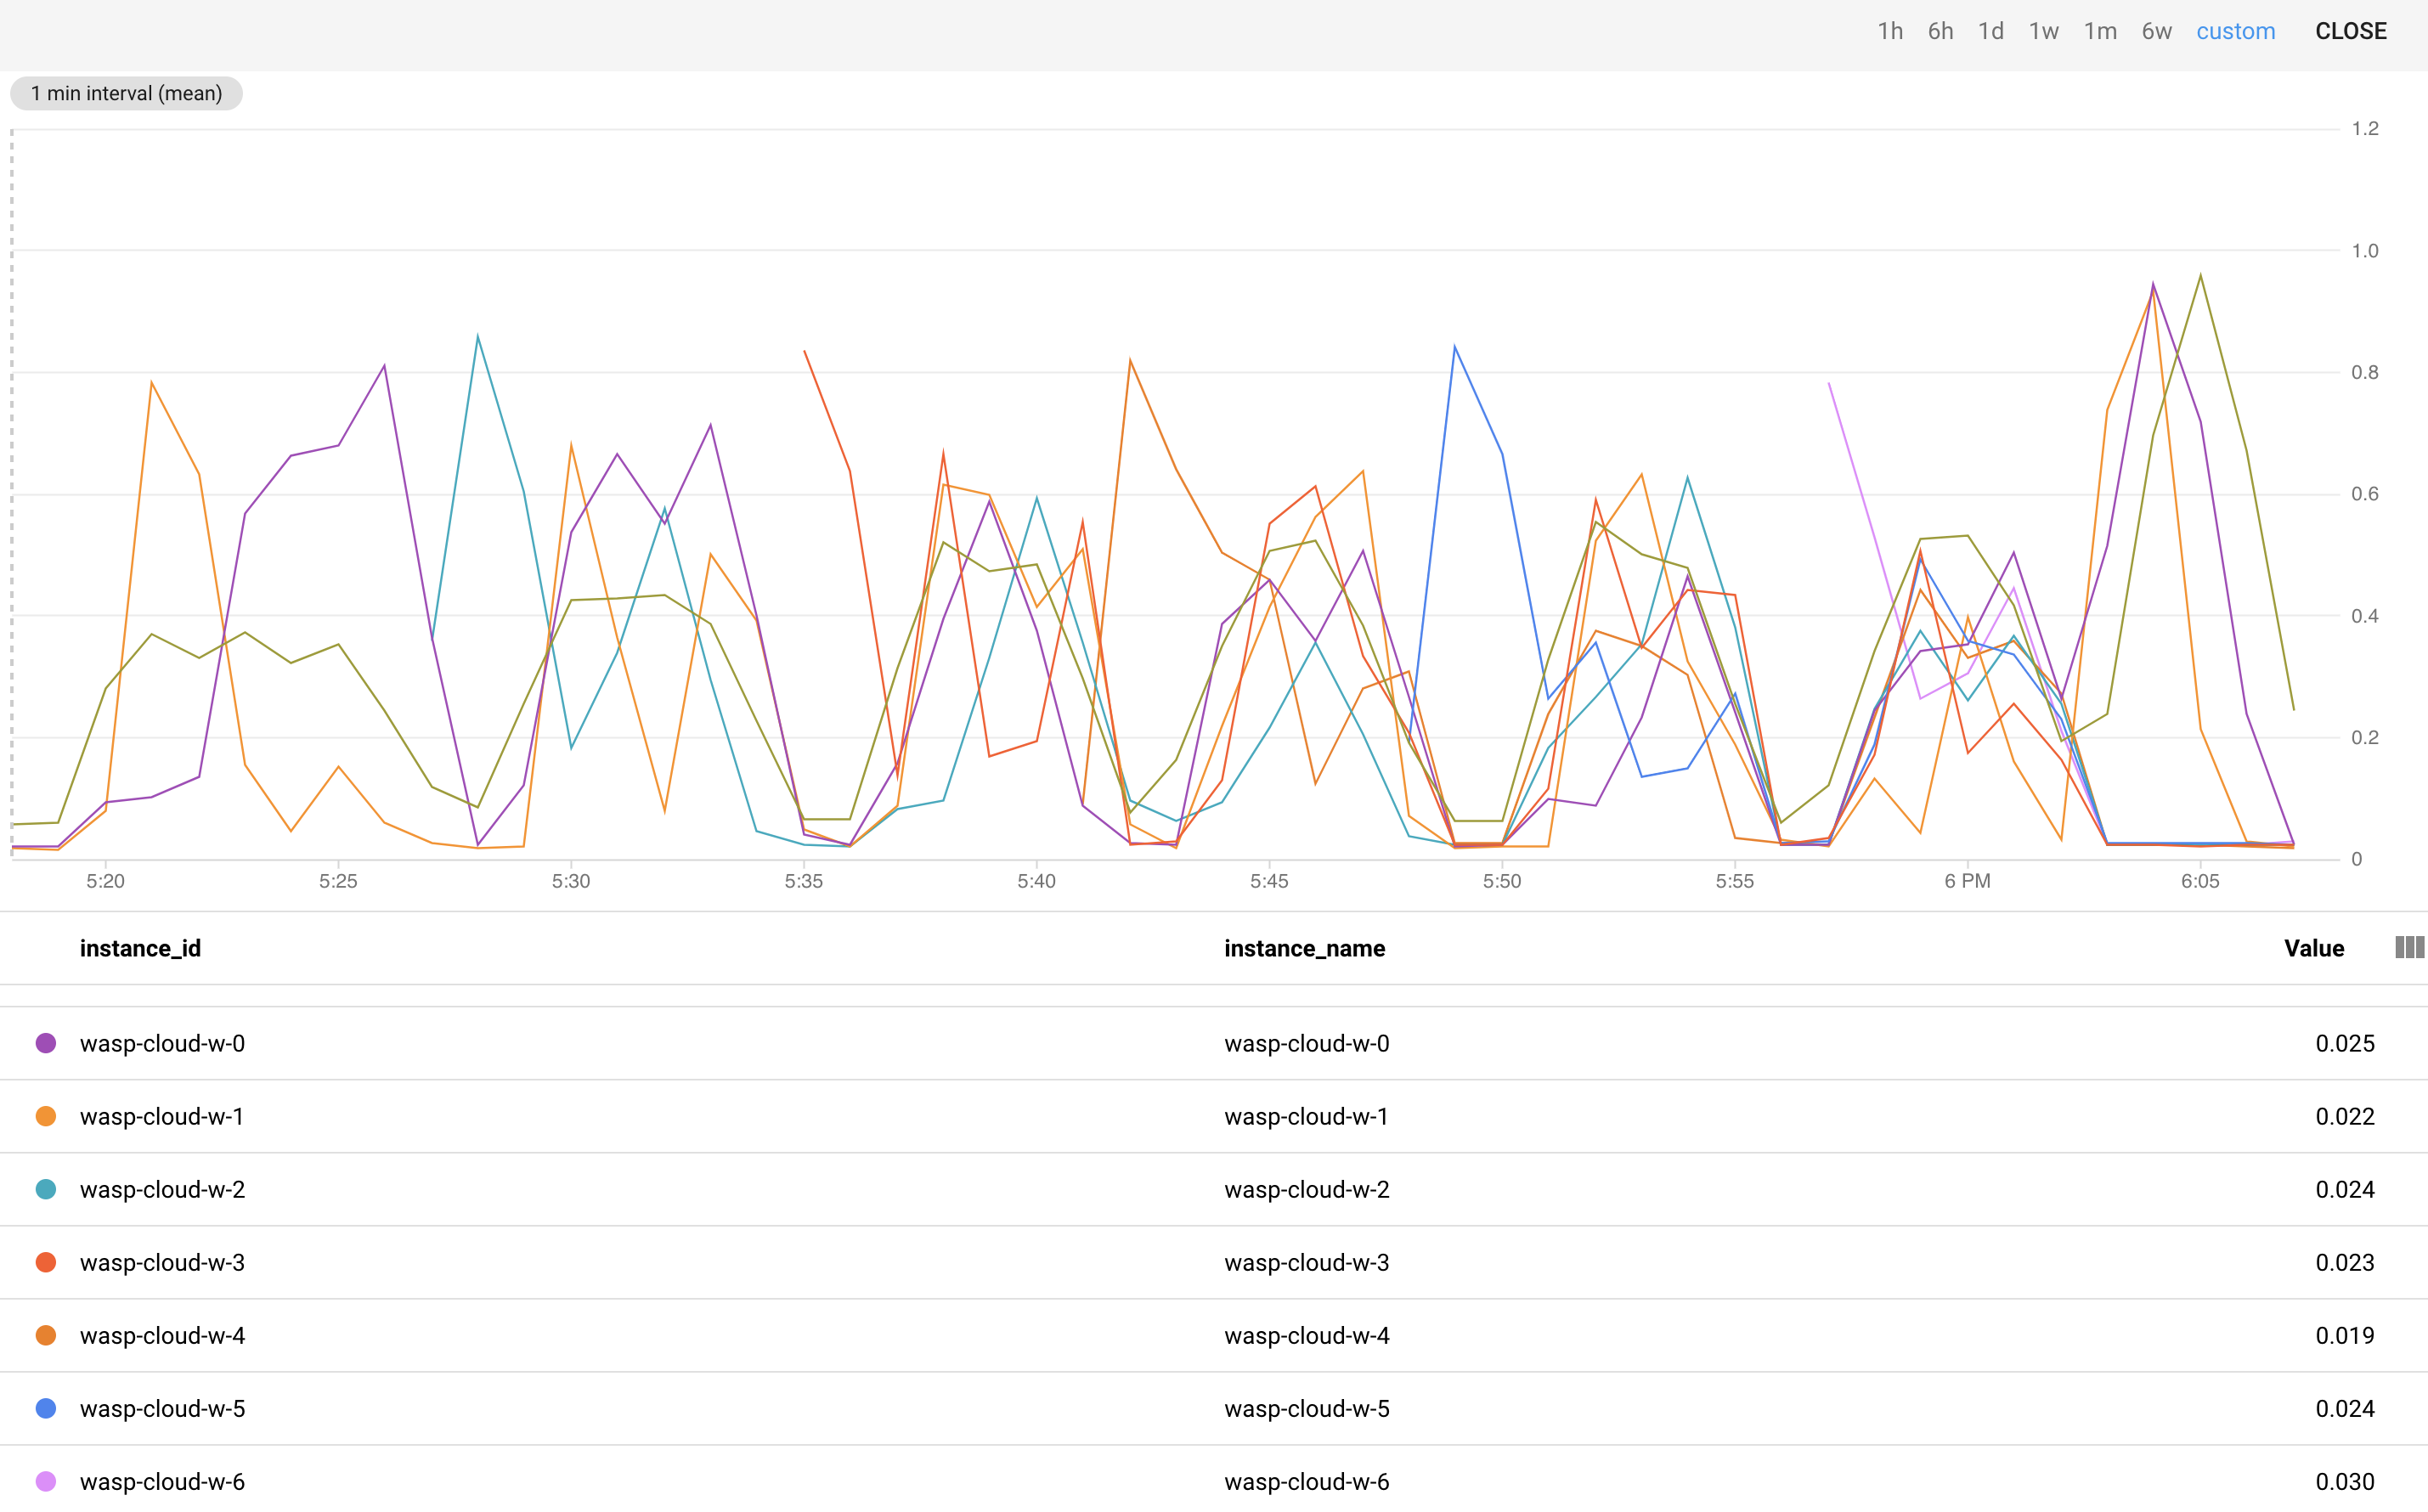
\includegraphics[width=0.8\textwidth]{img/multiply-cpu}
    \caption{Multipy Method – CPU Utilization}
    \label{fig:multiply-cpu}
\end{figure}

\begin{figure}[h]
    \centering
    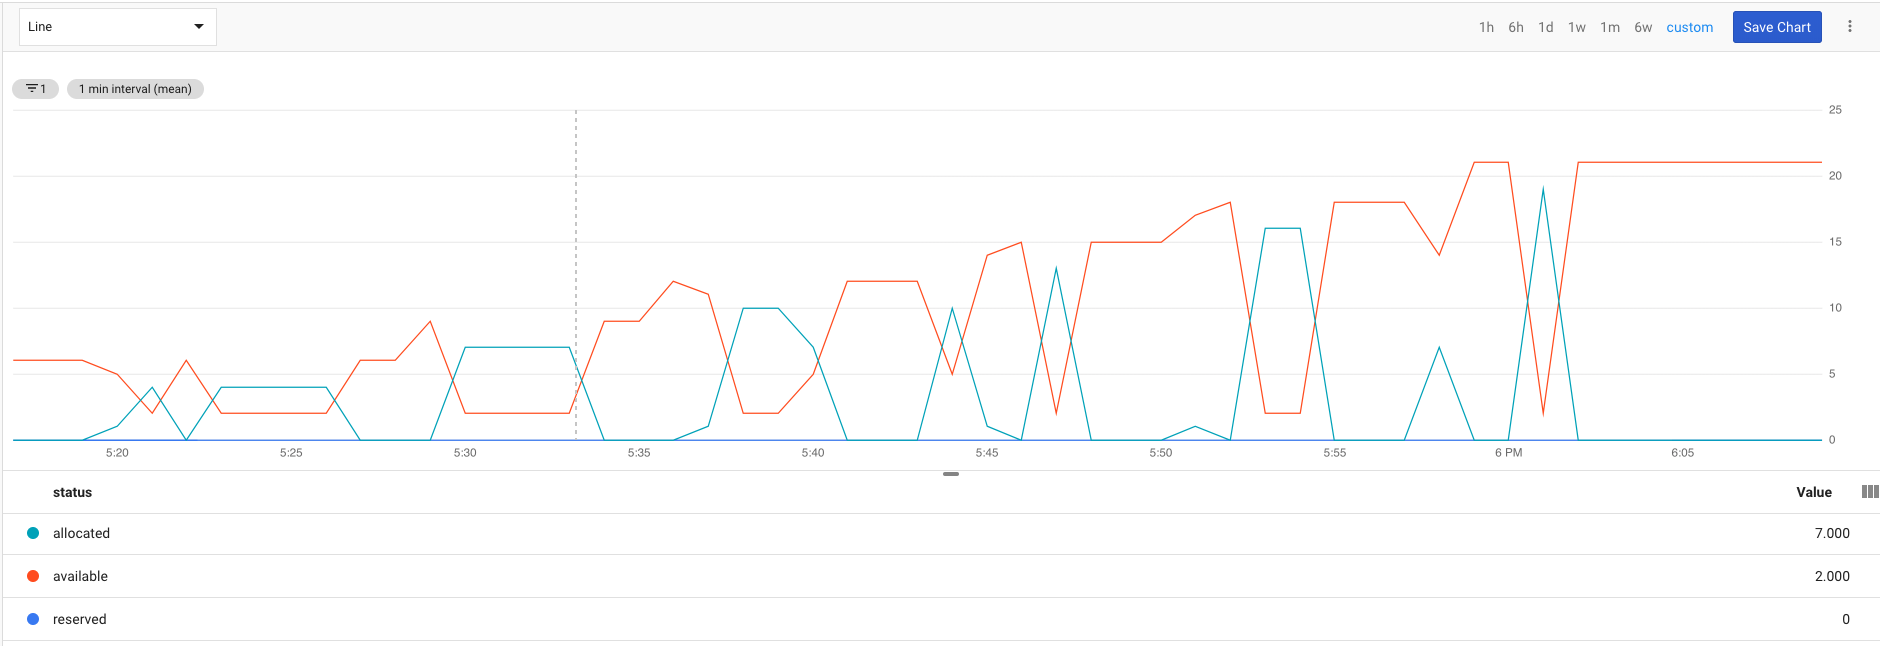
\includegraphics[width=0.8\textwidth]{img/multiply-memory}
    \caption{Multipy Method – Memory Utilization}
    \label{fig:multiply-mem}
\end{figure}


Figure~\ref{fig:svd} shows ...
%\begin{figure}[h]
%    \centering
%    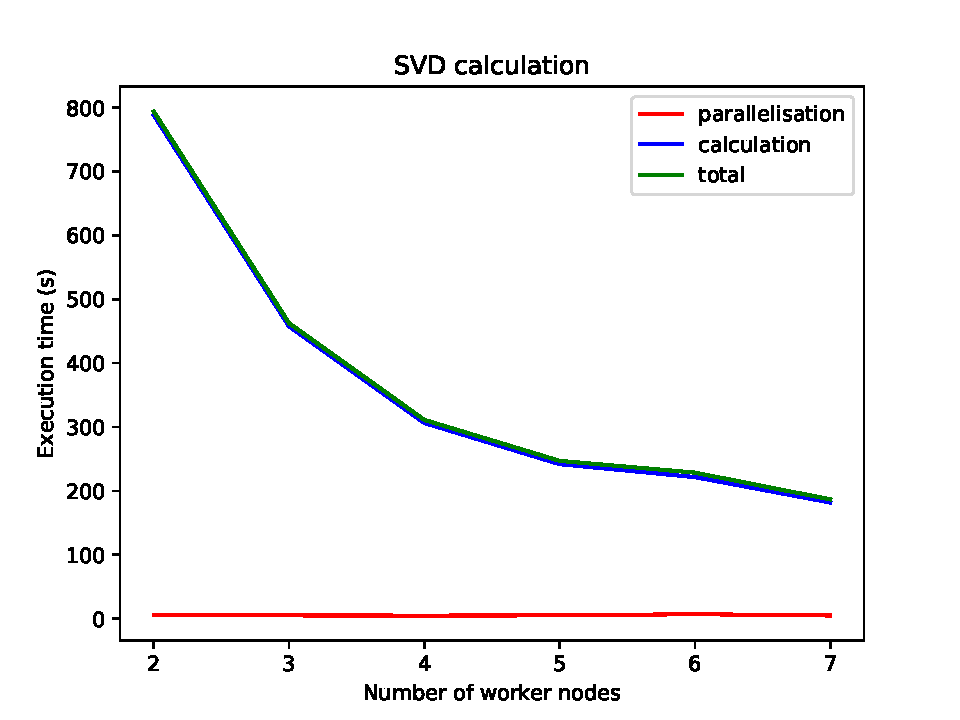
\includegraphics[width=\textwidth]{img/svd-speedup}
%    \caption{SVD Method – Speedup}
%    \label{fig:svd}
%\end{figure}

\begin{figure}[h]
    \centering
    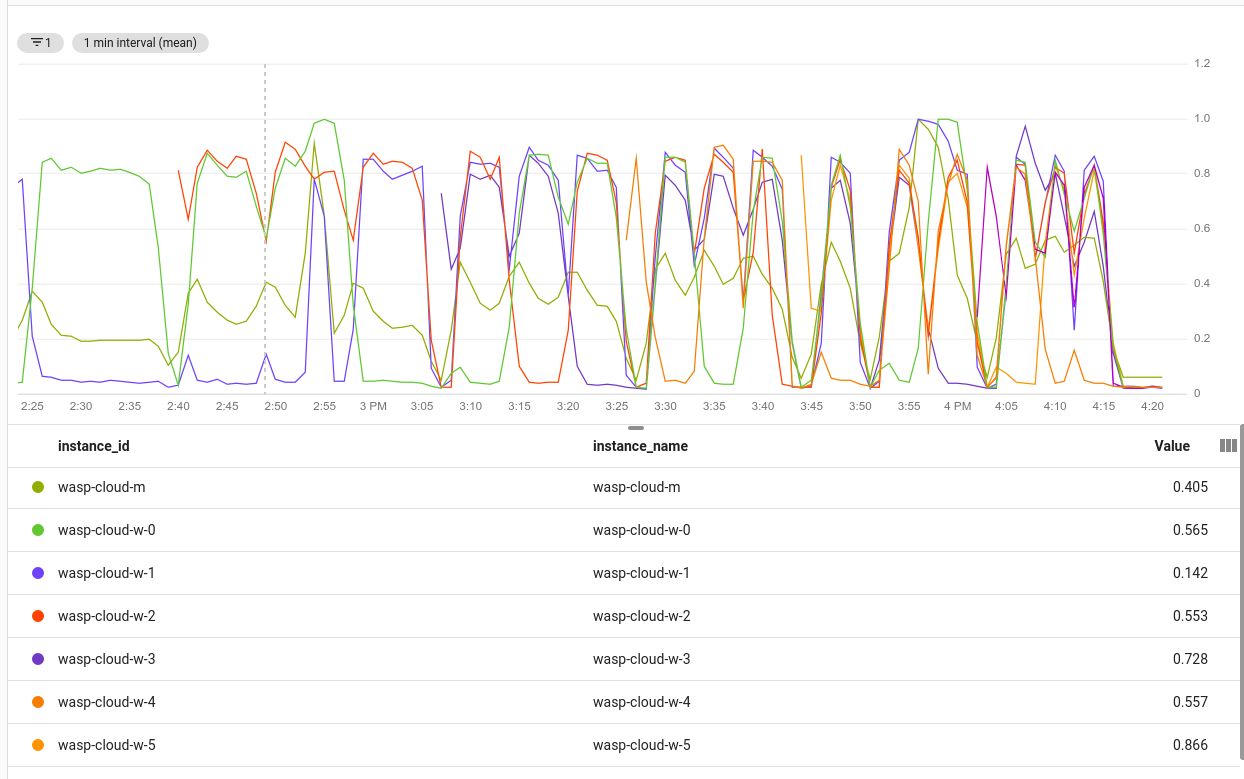
\includegraphics[width=0.8\textwidth]{img/svd-cpu}
    \caption{SVD Method – CPU Utilization}
    \label{fig:svd-cpu}
\end{figure}

\begin{figure}[h]
    \centering
    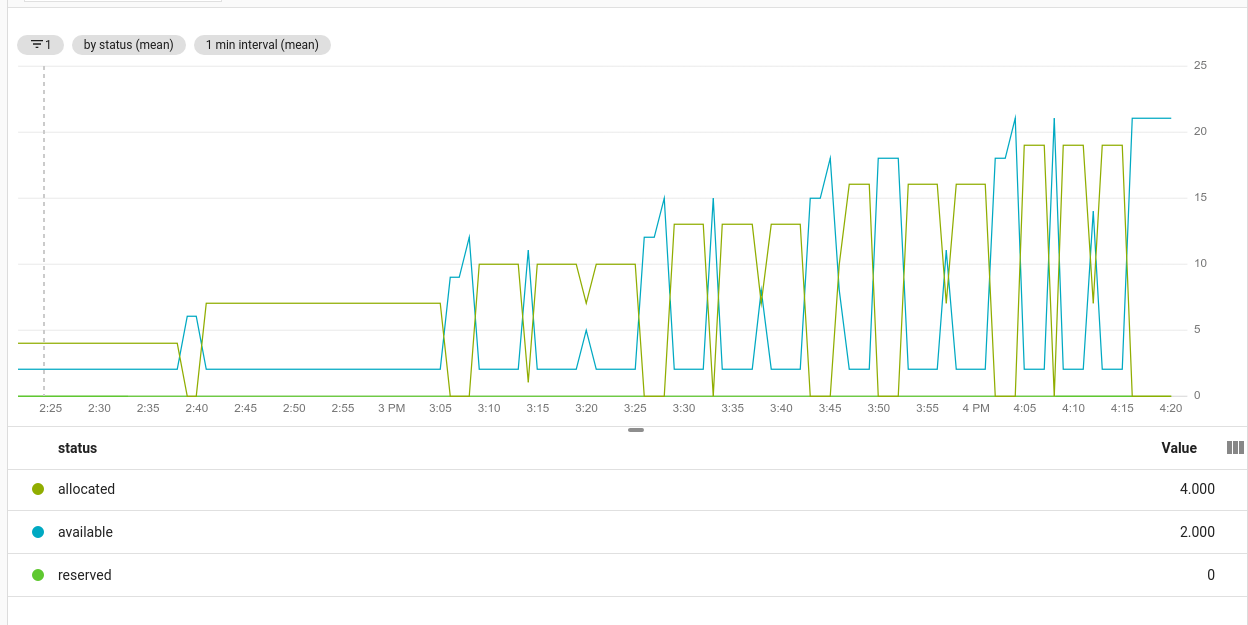
\includegraphics[width=0.8\textwidth]{img/svd-memory}
    \caption{SVD Method – Memory Utilization}
    \label{fig:svd-mem}
\end{figure}

\section{Lessons Learned}
We learned the use of the Google Dataproc the hard way by reverse-engineering an SDK in alpha status and conclude that using immature and undocumented API can be quite frustrating.

% Include a section where you comment on what you have learned, what did you think about the assignment, if you feel it is too easy, too hard, or something else. Please comment on what you liked an what you did not like.
I think the matrix operation part of the assignment lacks relevance in connection to the presented content at the cloud session in Umeå.
As this part is so important for the assignment, I miss an introduction into that topics (the referrenced paper fulfills that purpose only partially).
Trying to reverse-engineer poorly documented matrix operation APIs (which abstract the interesting distribution part anyways) does not contribute to the learning outcomes for a cloud course in my opinion.
I think it could be cool to formulate an assignment more open and incorporate use cases from different fields in the context of scaling out in the cloud (c.f., in the direction of the assignments for the software part of the course).

\bibliographystyle{IEEEtran}
\bibliography{cloud-linalg.bib}

\end{document}
